\documentclass[a4paper,12pt]{article} % тип документа
\usepackage[margin=1in]{geometry} % Поля

%  Русский язык
\usepackage[warn]{mathtext}
\usepackage[T2A]{fontenc}			% кодировка
\usepackage[utf8]{inputenc}			% кодировка исходного текста
\usepackage[english,russian]{babel}	% локализация и переносы
% Математика
\usepackage{amsmath,amsfonts,amssymb,amsthm,mathtools} 
\usepackage{wasysym}
%%%
\usepackage{graphicx}

\usepackage{tabularx}

\usepackage{gensymb} % знак градуса
\usepackage{enumitem} % изменить список enumerate
\usepackage{placeins} % \FloatBarrier

\renewcommand{\thesection}{\Roman{section}} 
\renewcommand{\thesubsection}{\roman{subsection}}


\begin{document}

\newcolumntype{Y}{>{\centering\arraybackslash}X} %new tabularx


%титул
\hrule 	
\medskip
\begin{raggedright}
{\large \textbf{Отчёт по работе 4.7.3}}
\\
\medskip
{\Large Поляризация} 
\\
\medskip
{\large Карташов Констанин Б04-005}
\medskip
\hrule
\medskip
\end{raggedright}


\section{Анотация}

\paragraph{Цель работы:} 
Ознакомление с методами получения и анализа поляризованного света.

\paragraph{Оборудование:}
\begin{itemize}
\renewcommand{\labelitemi}{$\triangleright$}
\itemsep0em
\item Оптическая скамья с осветителем,
\item Зелёный светофильтр,	
\item Два поляроида,
\item Чёрное зеркало,
\item Эбонитовая пластинка,
\item Стопа стеклянных пластинок,
\item Пластинки $\lambda/2$ и $\lambda/4$.
\end{itemize}


\medskip\hrule\medskip

\section{Теоретическая часть}

\subsection{Поляроид}

\paragraph{} Поляроид -- устройство пропускающее только компоненту света, соответствующую разрешённому направлению. Поляроид представляет собой тонкую пластинку, затемняющую проходящий свет.

\subsection{Двояко-преломляющая пластинка}

\paragraph{} Двояко-преломляющая пластинка -- тонка кристаллическая пластинка имеющая разные показатели преломления в зависимости от направления поля проходящей волны. Двояко-преломляющая пластинка имеет два взаимно перпендикулярных главных направления, первое <<медленное>> с наибольшей диэлектрической проницаемостью и второе <<быстрое>> с наименьшей.

При прохождении через пластинку компоненты электромагнитной волны совпадающие с главными осями приобретают сдвиг фаз. <<Толщина>> пластинки -- это количество длин волны соответствующее такому сдвигу фаз.

\subsection{Стопа Столетова}

\paragraph{} Стопа Столетова -- стопка из нескольких стеклянных пластинок, при прохождении через которую свет приобретает поляризацию перпендикулярную плоскости падения, а отражённый луч поляризован параллельно плоскости падения. Работы стопы Столетова основано на законе Брюстера.

\medskip\hrule\medskip

\section{Экспериментальная часть}

\subsection{Определение разрешённых направлений поляроида}

\begin{figure}[h]
\center
\begin{minipage}{0.49\textwidth}
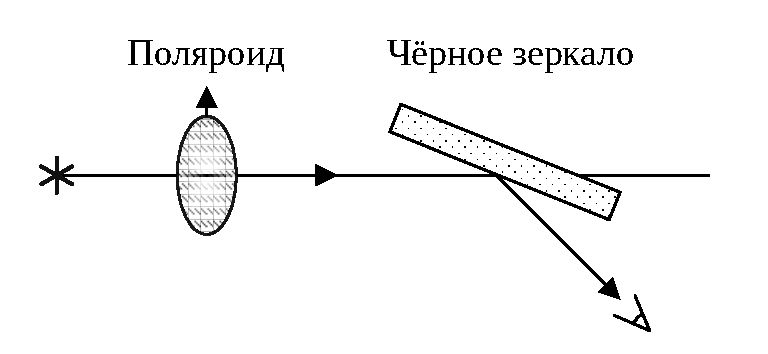
\includegraphics[width=\textwidth]{exp1.pdf}
\end{minipage}
\begin{minipage}{0.49\textwidth}
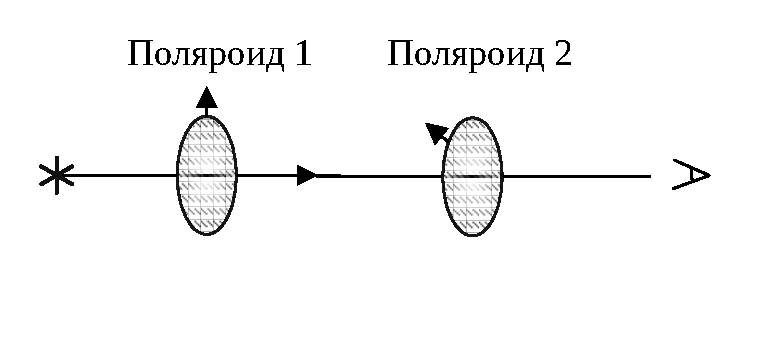
\includegraphics[width=\textwidth]{exp1_1.pdf}
\end{minipage}
\caption{Определение разрешённого направлений поляроида}
\label{fig:exp1}
\end{figure}

\paragraph{} Для определения разрешённый направлений поляроида установим на оптической скамье осветитель, поляроид, и чёрное зеркало. Поворачивая поляроид вокруг направления луча, а чёрное зеркало вокруг вертикальной оси, добьёмся наименьшей яркости отражения осветителя в зеркале (рис. \ref{fig:exp1}). 

При наименьшей яркости поляроид пропускает лучи с вертикальной поляризацией, так как отражённый от зеркала под углом Брюстера луч имеет горизонтальную поляризацию.

\paragraph{} Для определения разрешённого направления второго поляроида расположим на оптической скамье первый и второй поляроид. Поворачивая второй поляроид вокруг направления луча добьёмся наименьшей яркости проходящего через него луча.

При наименьшей яркости второй поляроид пропускает лучи с горизонтальной поляризацией, так как первый поляроид пропускает лучи с вертикальной поляризацией.

\subsection{Определение показателя преломления эбонита}

\begin{figure}[h]
\center
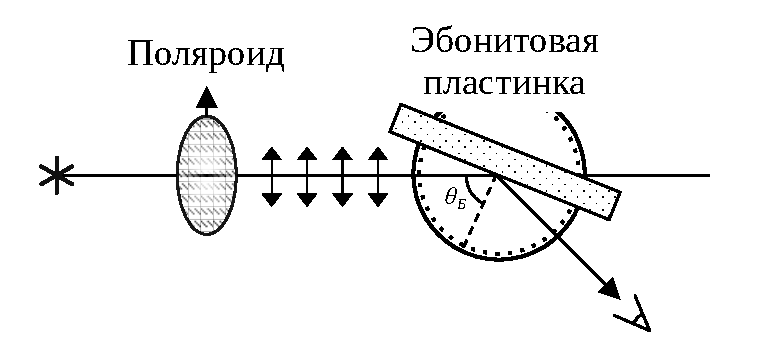
\includegraphics[width=0.5\textwidth]{exp2.pdf}
\caption{Определение показателя преломления эбонита}
\label{fig:exp2}
\end{figure}

\paragraph{} Поместим на оптическую скамью осветитель, поляроид и эбонитовую пластинку (рис. \ref{fig:exp2}). Выставим на поляроиде вертикальную поляризацию, зафиксируем на лимбе эбонитовой пластинки начало отчёта $\varphi_0 = 180\degree \pm 1 \degree$. 

Зафиксируем углы при которых на эбонитовой пластинке не видно отражения осветителя: $\varphi_1 = 226\degree \div 234 \degree$	. Повторим тоже самое измерение с зелёным световым фильтром: $\varphi_2 = 229 \degree \div 234 \degree$.

Вычтя начало отчёта получим оценку угла Брюстера: $\theta_\text{Б} \approx 49 \degree \div 53 \degree$. (Табличное значение $\theta_\text{Б} = 56 \degree \div 58 \degree$)

\subsection{Изучение поляризации в преломлённом и отражённом лучах}

\begin{figure}[h]
\center
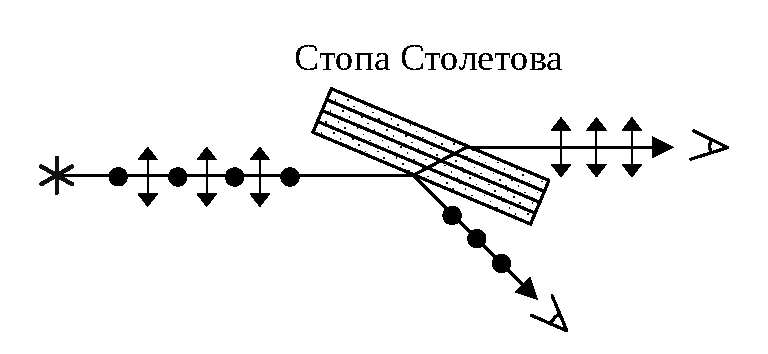
\includegraphics[width=0.5\textwidth]{exp3.pdf}
\caption{Поляризация в стопе Столетова}
\label{fig:exp3}
\end{figure}

\paragraph{} Поместим на оптическую скамью осветитель и скамью Столетова. Через поляроиды с известными разрешёнными направлениями посмотри на отражённый и прошедшие лучи. Видим, что отражённый луч поляризован горизонтально. Прошедший луч поляризован по больше мере вертикально с небольшой горизонтальной компонентой. (рис. \ref{fig:exp3})

\subsection{Определение главных направлений двояко-преломляющих пластин}

\begin{figure}[h]
\center
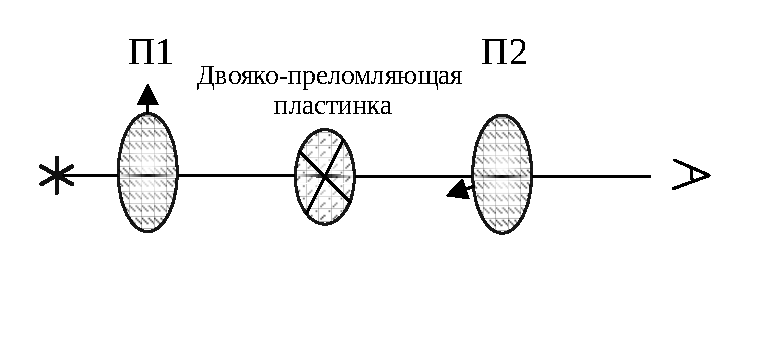
\includegraphics[width=0.5\textwidth]{exp4.pdf}
\caption{Определение главных направлений двояко-преломляющей пластины}
\label{fig:exp4}
\end{figure}


\paragraph{} Поместим на оптическую скамью два оптических фильтра. Выставим направления первого и второго поляроида -- вертикально и горизонтально соответственно. Теперь поочерёдно поместим двояко-преломляющие пластинки между поляроидами. Когда яркость проходящего света минимальна -- главное направление пластинки совпадает с направлениями поляроидов. Для обоих пластинок зафиксируем главные направления. (рис. \ref{fig:exp4})

\subsection{Выделение пластинок $\boldsymbol\lambda / \mathbf{2}$ и $\boldsymbol\lambda / \mathbf{4}$}

\paragraph{} Добавим к прошлому схеме зелёный цветовой фильтр. Поочерёдно поместим пластинки между поляроидами так, чтобы главные направления не совпадали с направлением первого поляроида. Теперь будем вращать второй поляроид и в зависимости от наблюдаемого эффекта установим тип пластинки: 

Для пластинки $\lambda/4$ яркость проходящего света почти не будет меняться, для пластинки $\lambda/2$ яркость будет меняться так же, как при отсутствии пластинки (однако направления второго поляроида для максимальной и минимальной яркости будут отличаться).

\subsection{Определение <<быстрой>> и <<медленной>> оси в пластинке $\boldsymbol\lambda / \mathbf{4}$}

\paragraph{} Поместим на оптическую скамью два скрещённых поляроида и пластинку $\lambda$ с главным направлением под углом $45\degree$ к осям поляроидов. Посмотрев через поляроиды увидим, что пластинка имеет пурпурный цвет. Теперь поместим пластинку $\lambda / 4$ между поляроидами так, чтобы её главные направления совпадали с главными направлениями пластинки $\lambda$.

Теперь снова посмотрим через поляроид. Видим, что пластинка имеет голубоватый цвет, значит быстрые направления пластинок $\lambda/4$ и $\lambda$ совпали.

Чтобы убедится, повернём пластинку  $\lambda/4$ на $90\degree$. Видим, что пластинка имеет оранжевый цвет, значит быстрые направления не совпали.

\subsection{Интерференция поляризованных лучей}

\begin{figure}[h]
\center
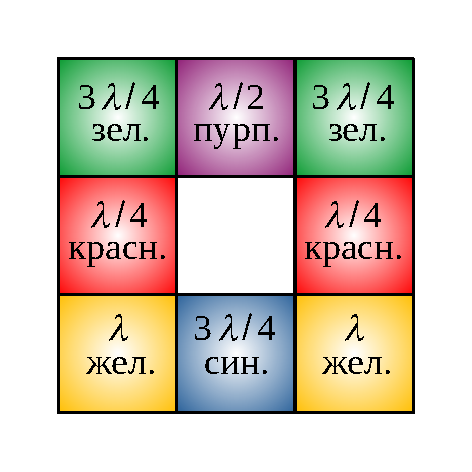
\includegraphics[width=0.3\textwidth]{plast.pdf}
\caption{<<толщина>> пластинки и соответствующий цвет}
\label{fig:plast}
\end{figure}

\paragraph{} Поместим между двумя скрещёнными поляроидами мозаичную пластинку состоящую из четырёх полосок слюды, лежащих по сторонам квадрата (две полоски $\lambda/2$, одна $\lambda/4$ и одна $3\lambda/4$).  Цвета и <<толщина>> приведены на (рис. \ref{fig:plast})

\paragraph{} Будем вращать пластинку вокруг направления луча, и наблюдать за видимым эффектом. Видим, что цвета не меняются, при этом меняется интенсивность света.

\paragraph{} Поместим пластинку под углом $45\degree$ и будем вращать второй поляроид. Видим, что меняются цвета пластинки, а интенсивность не изменяется.

\medskip\hrule\medskip

\section{Выводы}

\begin{enumerate}
\item Определили разрешённое направление поляроида пользуясь законом Брюстераю, и пользуясь поляроидом с известным разрешённым направлением.
\item Проверили теорию Брюстера на эбонитовой пластинке. Измеренное значения угла брюстера оказалось на $3\degree \div 9 \degree$ меньше теоретического значения. Это может быть связано со смещённым началом отсчёта и неровностями на поверхности эбонита.
\item Измерили поляризацию света в стопе Столетова.
\item Определили главные направления и <<толщину>> двояко-преломляющих пластин.\
\item Определили <<быструю>> и <<медленную>> ость в пластинке $\lambda/4$.
\item Пронаблюдали интерференцию поляризованных лучей на двояко-преломляющих пластинках с разной толщиной.
\end{enumerate}

\medskip\hrule\medskip

\end{document}
